\clearpage
\subsection{Which physical failures dominate the screen?}
The metallic lower bound resolves the gap and both edge penalties jointly. For a metal with common edge $t$, the vertical distance above the following curve is exactly the formation-energy penalty, up to the supplied rounding:
\[
 B(t)=7.84+[ (5.73-t)/0.5 ]_+^2+[(t-4.50)/0.5]_+^2 .
\]
Moving the common edge to the left alleviates the CBM violation while increasing the VBM violation. Moving it to the right has the opposite effect. Their thresholds are separated by 1.23 eV. Figure~\ref{fig:regimes} shows why neither edge adjustment can compensate for zero gap.

\begin{figure}[ht]
\centering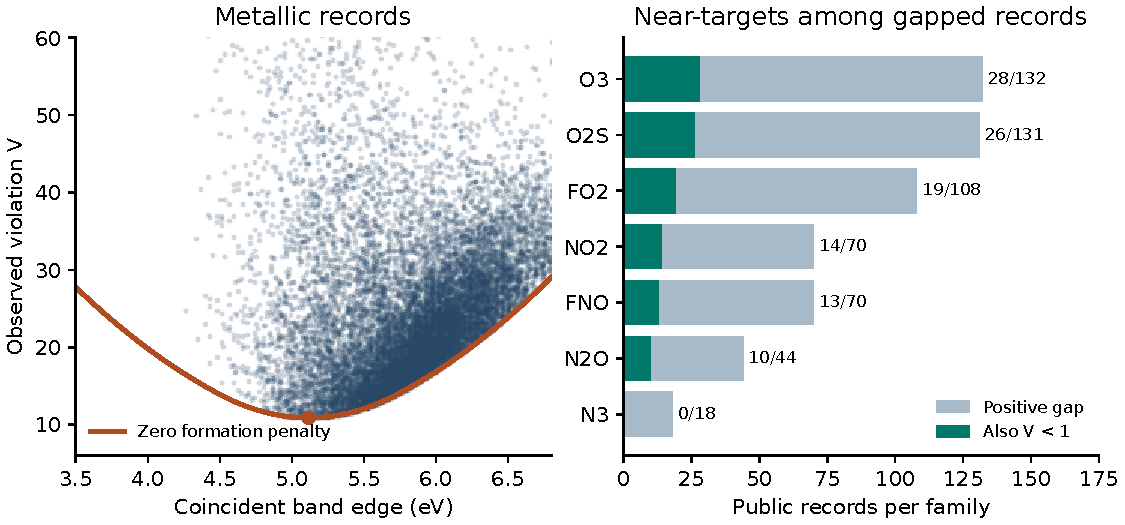
\includegraphics[width=\linewidth]{figures/physical_regimes.pdf}
\caption{Left, labeled metallic records from files 02 and 03 in the displayed edge and violation window. The curve gives $B(t)$ and the dot its minimum. Right, each family has 2,175 labeled records. Numerators count $V<1$ records and denominators count positive-gap records.}\label{fig:regimes}
\end{figure}

Positive gap narrows the public screen from 15,225 records to 573 and retains all 110 with $V<1$. Even with the true gap known, only $110/573=19.2\%$ of the gapped records pass this relaxed test. In O3, 28 of 132 gapped compositions have $V<1$. In NO2, the ratio is 14 of 70, and in N3 none of 18 passes. These counts are descriptive. In particular, the hidden set was constructed to contain the exact targets, which changes the interpretation of any full-population prevalence estimate.

At inference the gate supplies only an estimated probability. In Eq.~\eqref{eq:mix}, an increase $\delta$ in the predicted metallic probability increases the predicted score by $\delta(f_0^\prime-f_+^\prime)$ with the clipped branch estimates held fixed. The effect is greatest when the two branches disagree. This is why a confidently wrong metallic assignment can hide a promising material. Conversely, a candidate assigned high positive-gap probability still has to survive its branch's estimated formation and edge penalties. The validation experiment below tests the combined effect in the order in which materials would be checked.

